\chapter{Details of the~method}\label{chap:details}

In this section, we describe the~details of the~method, namely how the~target mip-maps are constructed and what the~prediction operator $\opnorm{P}{}$ looks like.

The~down-sampling of the~mip-maps can be performed by any form of averaging. As we saw in the~previous chapter, the~maximum absolute error does not depend on how the~mip-maps look, as long as they contain valid values. However, the~way the~mip-maps are constructed affects the~compression ratio. Moreover, various mip-map constructions produce different visual artifacts. In terms of the~visual artifacts, the~best way to down-sample a mip-map is to just average the~four neighboring pixels [2n, 2n+1], [2n, 2n+1] at $\lnorm{i+1}$ into [n][n] at $\lnorm{i}$.

In the~previous section, we made a simplification claiming that a~decompressed mip-map $\ldot{i+1}$ is constructed from the~previous $\ldot{i}$ in just one step (eq. \ref{eq:nextLevel}). We did that in order to emphasize the~fact, that $maxdev(\ldot{i+1}, \lnorm{i+1}) < \objnorm{D}{}$. In fact, three such steps happen. Nevertheless, the~residuals are checked after each of these steps and all the~predictions are made from the~decompressed values, so the~maximum error bound is still kept. So, when we construct the~following decompressed mip-map, every pixel $p$ from $\ldot{i}$ is substituted by four pixels in $\ldot{i+1}$ as shown in Fig.~\ref{fig:subst}. 

\begin{figure}
	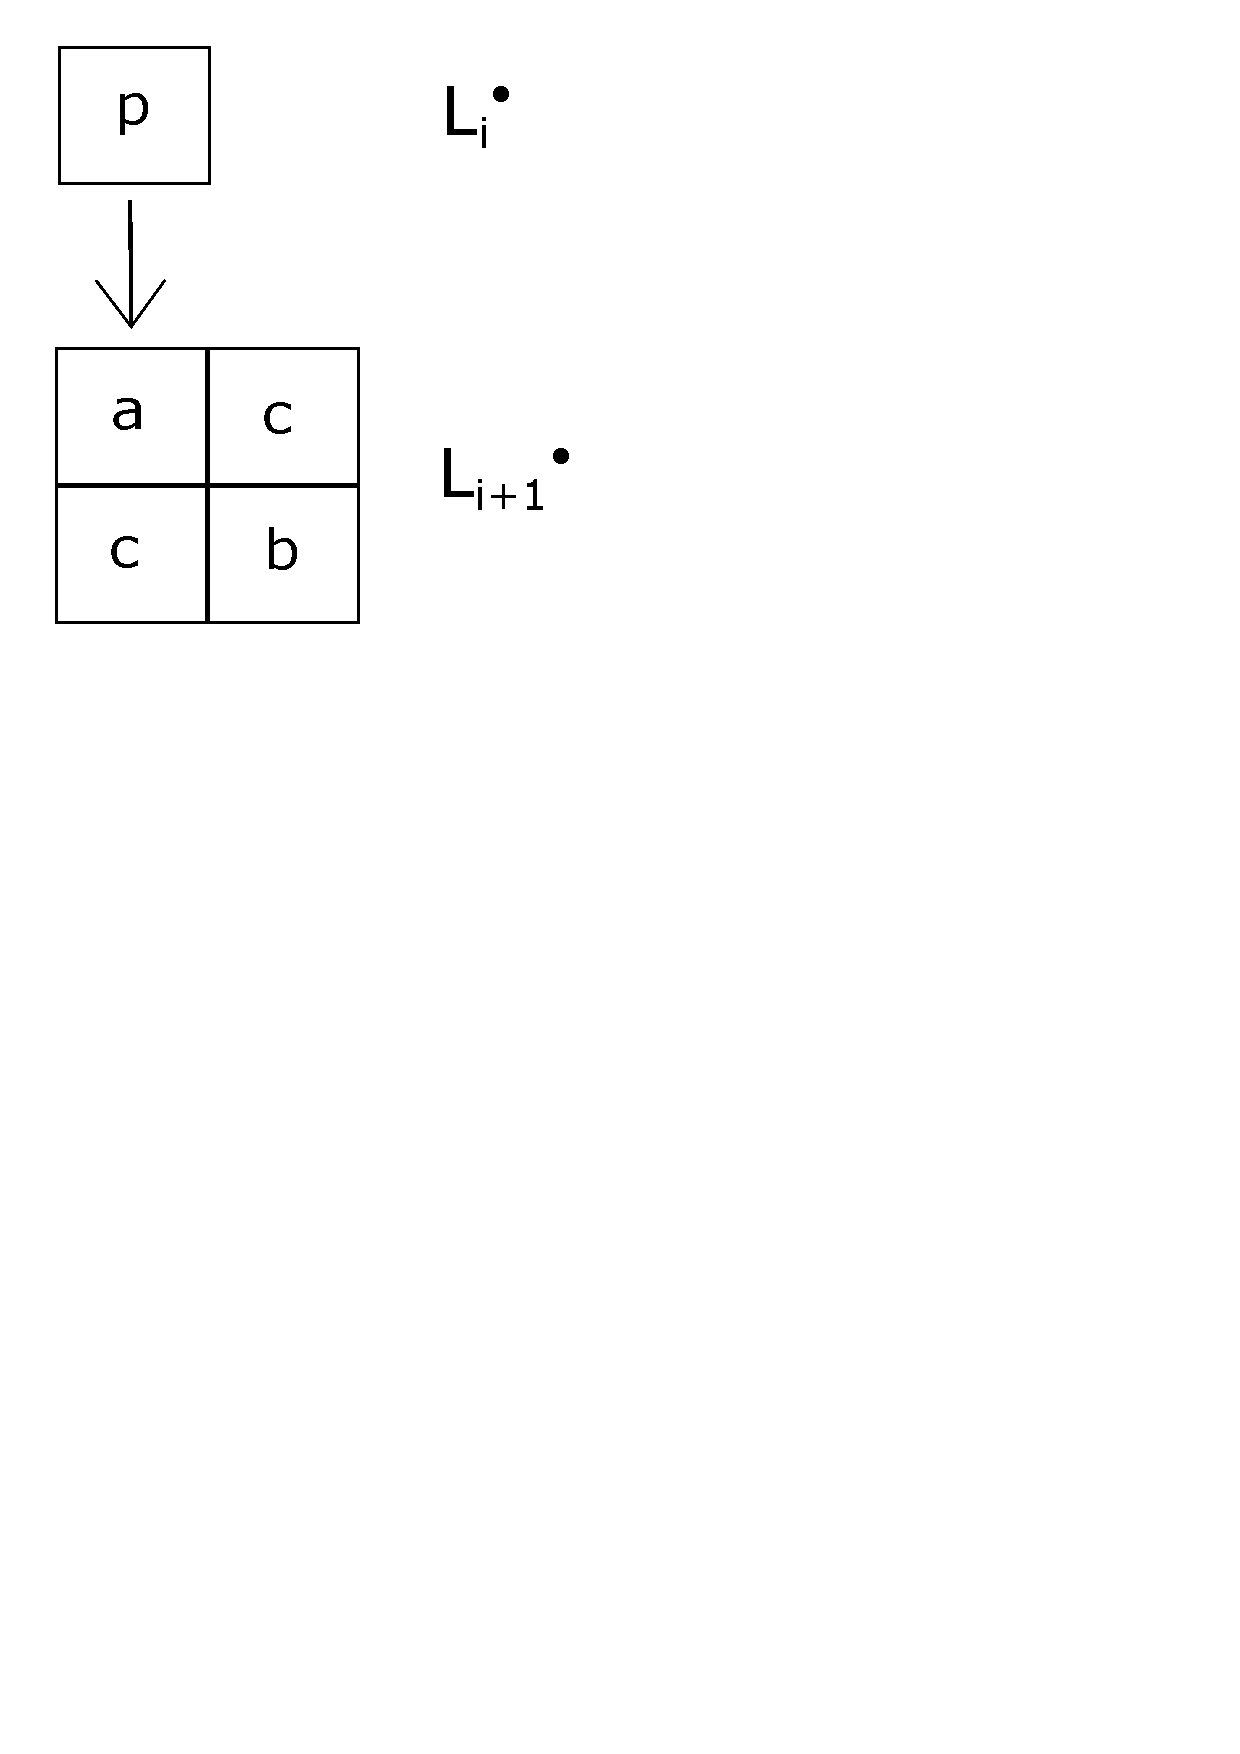
\includegraphics[trim={0 19cm 11cm 0}, clip, width=0.28\textwidth]{figures/subst.pdf}\centering
	\caption{Substitution of a~pixel p from $\ldot{i}$ by four children in $\ldot{i+1}$}
	\label{fig:subst}
\end{figure}

The~first one of them, labeled $a$, is predicted directly from $\ldot{i}$ by a~simple prediction operator $\opnorm{P}{a}(\ldot{i}) = p$. Following this, the~residuals $\objnorm{E}{a}$ and $\objdot{E}{a}$ are computed according to the~target value $a_t$ in $\lnorm{i+1}$ and $a$ is assigned the~final value $a\bullet$ (eq. \ref{eq:a}). It holds that  $maxdev(a\bullet, a_{t}) \leq \objnorm{D}{}$.

$$\objnorm{E}{a} = a_t - p$$
$$\objdot{E}{a} = \opnorm{Q}{D}(\objnorm{E}{a})$$
\begin{equation}
\label{eq:a}
a\bullet = p + \objdot{E}{a}
\end{equation}

The~second one of them, labeled $b$, is predicted from the~pixels $a\bullet$ in $\ldot{i+1}$ by the~straight-oriented order 2 Neville interpolating filter (fig. \ref{fig:bcomp}), just like the~border values are predicted in C-BDAM. A~similar computation of residuals $\objnorm{E}{b}$ and $\objdot{E}{b}$ then follows according to the~target value $b_t$ from $\lnorm{i+1}$ and $b$ is assigned the~final value $b\bullet$ (eq. \ref{eq:b}).

\begin{figure}
	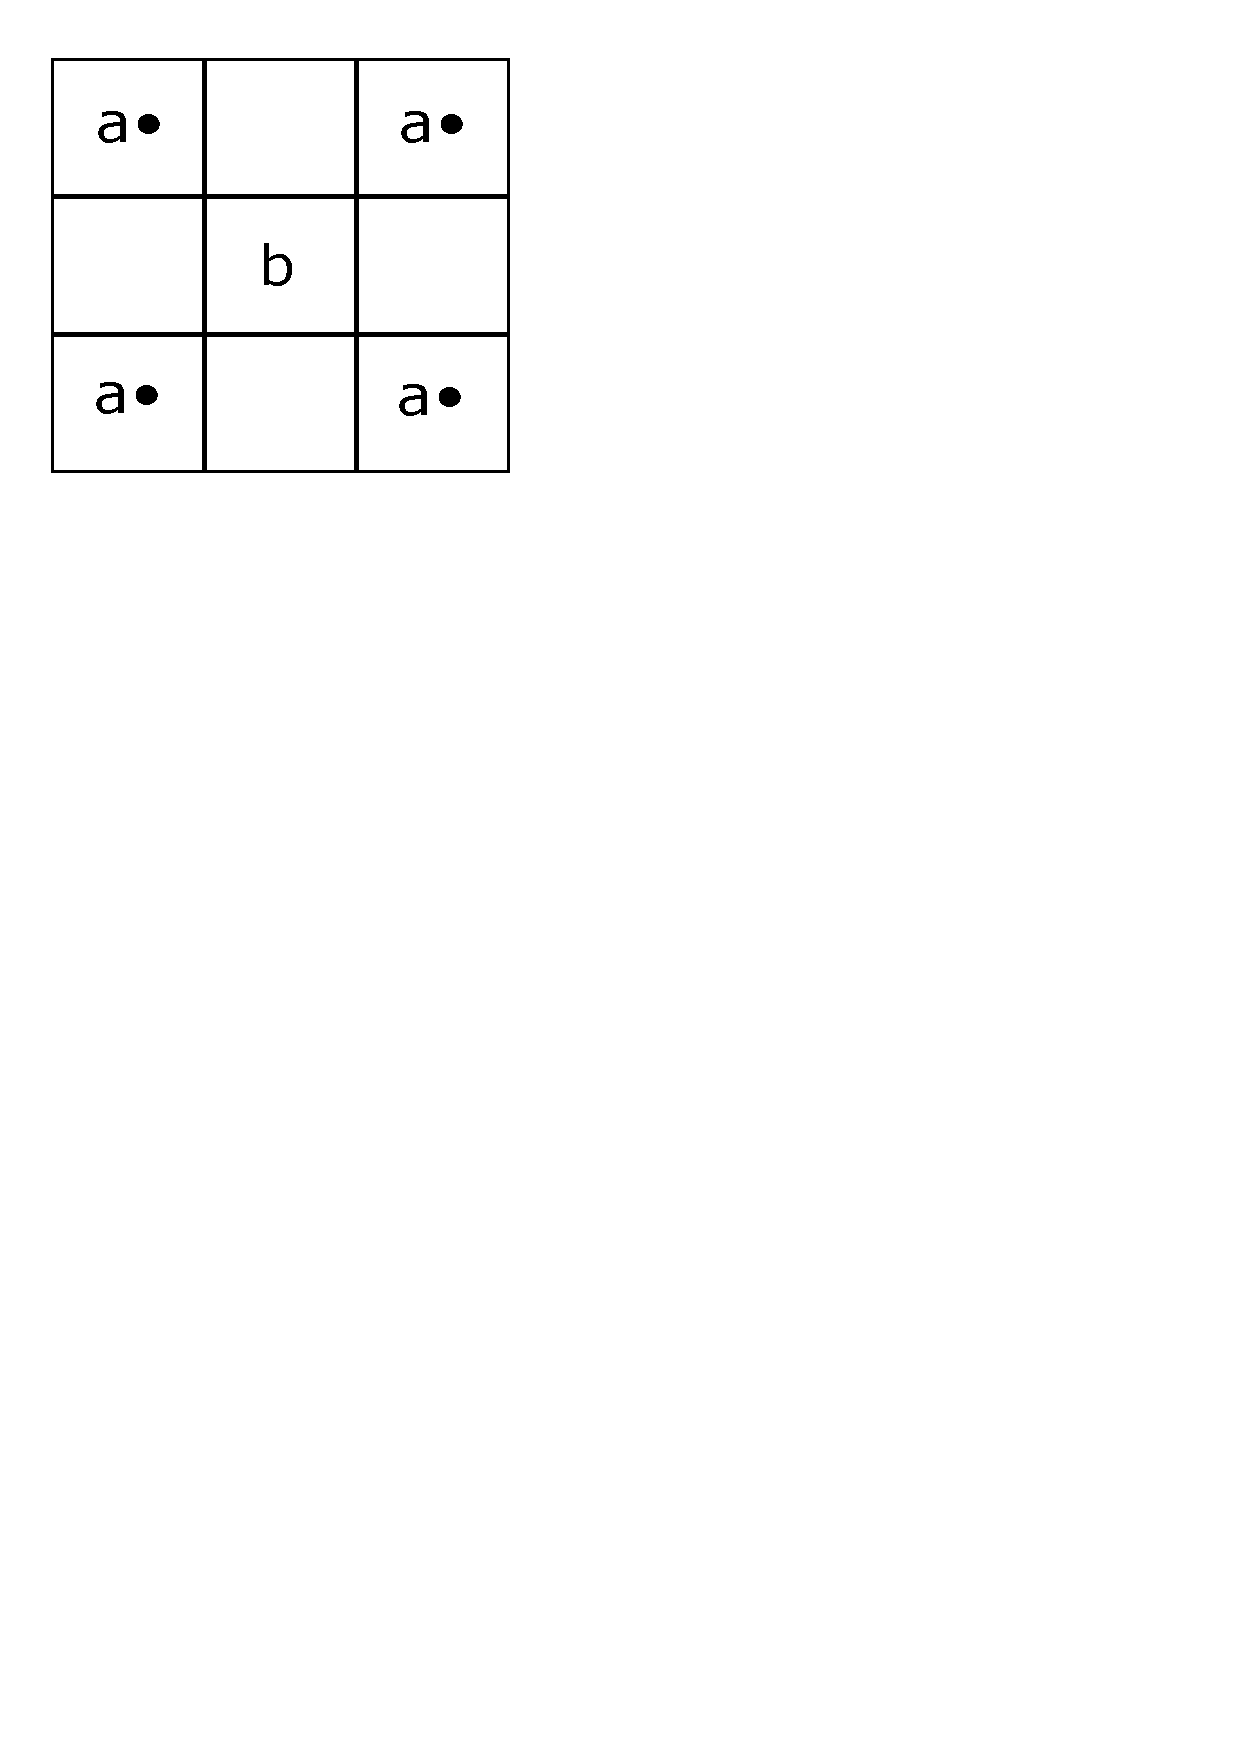
\includegraphics[trim={0 21cm 10cm 0}, clip, width=0.3\textwidth]{figures/bcomp.pdf}\centering
	\caption{The~prediction of $b$ - $\opnorm{P}{b}(\ldot{i+1})$ - is the~average of all the~displayed $a\bullet$}
	\label{fig:bcomp}
\end{figure}

$$\objnorm{E}{b} = b_t - \opnorm{P}{b}(\ldot{i+1})$$
$$\objdot{E}{b} = \opnorm{Q}{D}(\objnorm{E}{b})$$
\begin{equation}
\label{eq:b}
b\bullet = \opnorm{P}{b}(\ldot{i+1}) + \objdot{E}{b}
\end{equation}

The~cases when the~filter comes out of the~image are handled by a~specific mirror extension (fig. \ref{fig:bborders}). Unlike C-BDAM, where the~order 4 Neville filter is used for the~interior values, in this method, the~order 2 filter is used even for the~interior values in order to increase the~speed. As an additional optimization, the~interpolation with the~order 2 filter can be easily cached during horizontal traversal. Moreover, using the~order 4 filter made the~compression ratio slightly better - probably because it predicts hills and walleys more accurately, but made the~quality of the~reconstructed heightmap worse - it produced sharper artifacts on the~borders of smooth gradient terrain blocks (Fig.~\ref{fig:artifs_border}) and near sharp terrain changes (Fig.~\ref{fig:artifs_sharp_change}).

\begin{figure}
	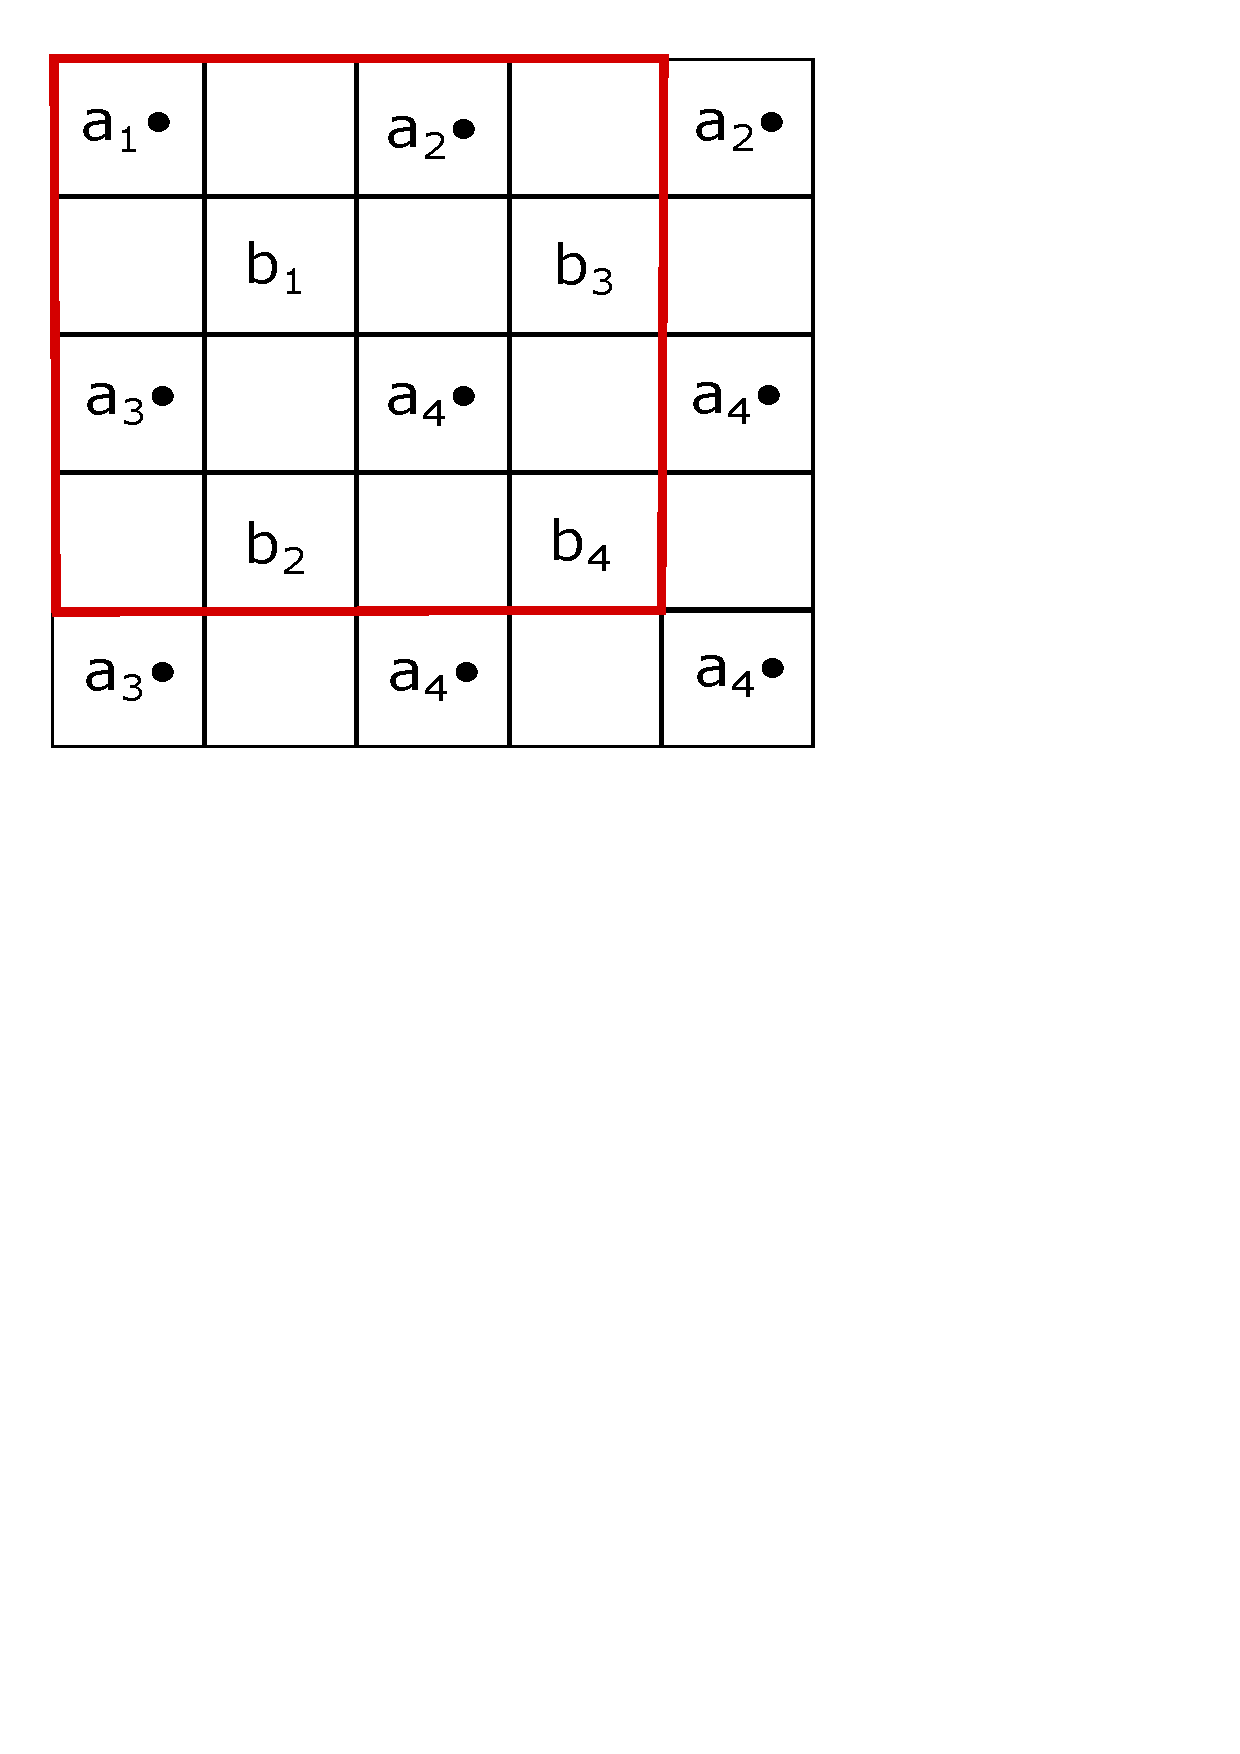
\includegraphics[trim={0 17cm 5cm 0}, clip, width=0.4\textwidth]{figures/extb.pdf}\centering
	\caption{Handling of border cases in the~computation of $\opnorm{P}{b}(\ldot{i+1})$ - the~red line represents the~border.}
	\label{fig:bborders}
\end{figure}

\newcommand{\incimg}[3]{\includegraphics[width=#1px, height=#2px]{#3}}
\newcommand{\incartifborder}[1]{\incimg{95}{70}{#1}}

\begin{figure}
	Original \incartifborder{figures/artif_orig0.png}
	\incartifborder{figures/artif_orig1.png}\\
	Order 2~~\incartifborder{figures/artif_four0.png}
	\incartifborder{figures/artif_four1.png}\\
	Order 4~~\incartifborder{figures/artif_twelve0.png}
	\incartifborder{figures/artif_twelve1.png}\\
	\caption{Two examples of different artifacts caused by order 2 and order 4 filters at the~border of smooth gradient terrain - the~first row shows the~target heightmaps, the~second row shows the~same heightmaps compressed with the~order 2 filter, the~third row with the~order 4 filter.}
	\label{fig:artifs_border}
\end{figure}

\newcommand{\incartifchange}[1]{\incimg{95}{95}{#1}}

\begin{figure}
	Original \incartifchange{figures/artif_change_orig0.png}
	\incartifchange{figures/artif_change_orig1.png}\\
	Order 2~~\incartifchange{figures/artif_change_four0.png}
	\incartifchange{figures/artif_change_four1.png}\\\
	Order 4~~\incartifchange{figures/artif_change_twelve0.png}
	\incartifchange{figures/artif_change_twelve1.png}\\
	\caption{Two examples of different artifacts caused by order 2 and order 4 filters at a~sharp terrain change - the~first row shows the~target heightmaps, the~second row shows the~same heightmaps compressed with the~order 2 filter, the~third row with the~order 4 filter. The~values in the~original images range from 0 to 16 and the~maximum deviation of the~compression is 9.}
	\label{fig:artifs_sharp_change}
\end{figure}

The~reason for these artifacts is that while the~predictions are close enough to the~real terrain (their~quantized residuals are zeroes), the~reconstructed values might be systematically above/under the~terrain. But as soon as one prediction is a bit further from the~terrain than those at the~adjacent pixels, its residual is quantized to a~non-zero value and the~reconstructed value might flip to the~other side of the~terrain, producing a~visual artifact. This often happens when smooth terrain is followed by a~sharp change. The~prediction operator might then predict different values near this change, as it reaches out to the~area behind the~change (Fig.~\ref{fig:artifs_theory2}, \ref{fig:artifs_theory}). This spike is then propagated to the~next levels, but still within the~maximum error bound. The~mirroring at the~borders produces such sharp changes, too, in a different, more complex way. However, some better form of mirroring might sort this out.

\begin{figure}
	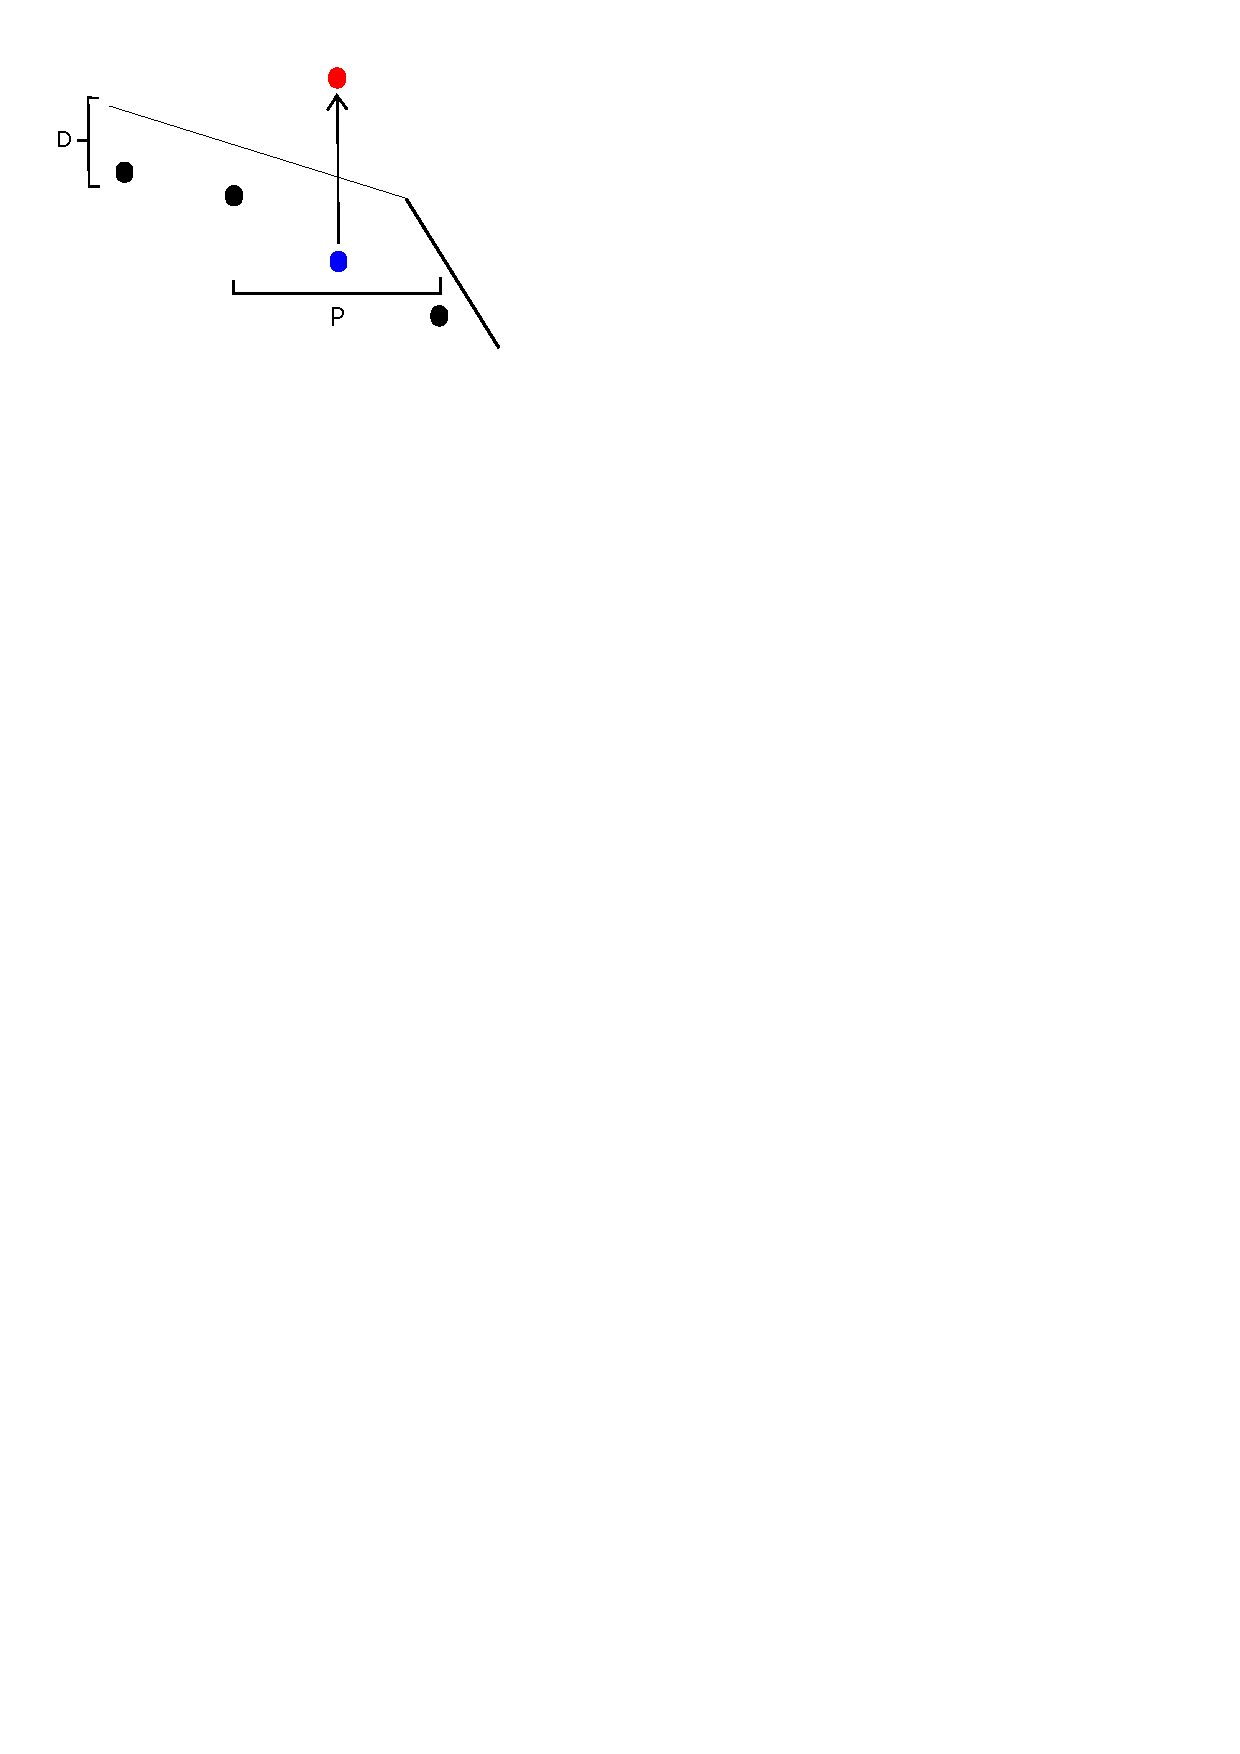
\includegraphics[trim={0 24cm 7cm 0}, clip, width=0.45\textwidth]{figures/artifs_theory.pdf}\centering
	\caption{The~illustration of how an~artifact occurs - the~black predictions are within the~maximum-error bound $D$, so they are equal to the~reconstructed values, but the~blue one is not. Because a~uniform quantizer is used, the~blue prediction is shifted by $2D - 1$ to the~top, creating an~artifact.}
	\label{fig:artifs_theory2}
\end{figure}

\begin{figure}
	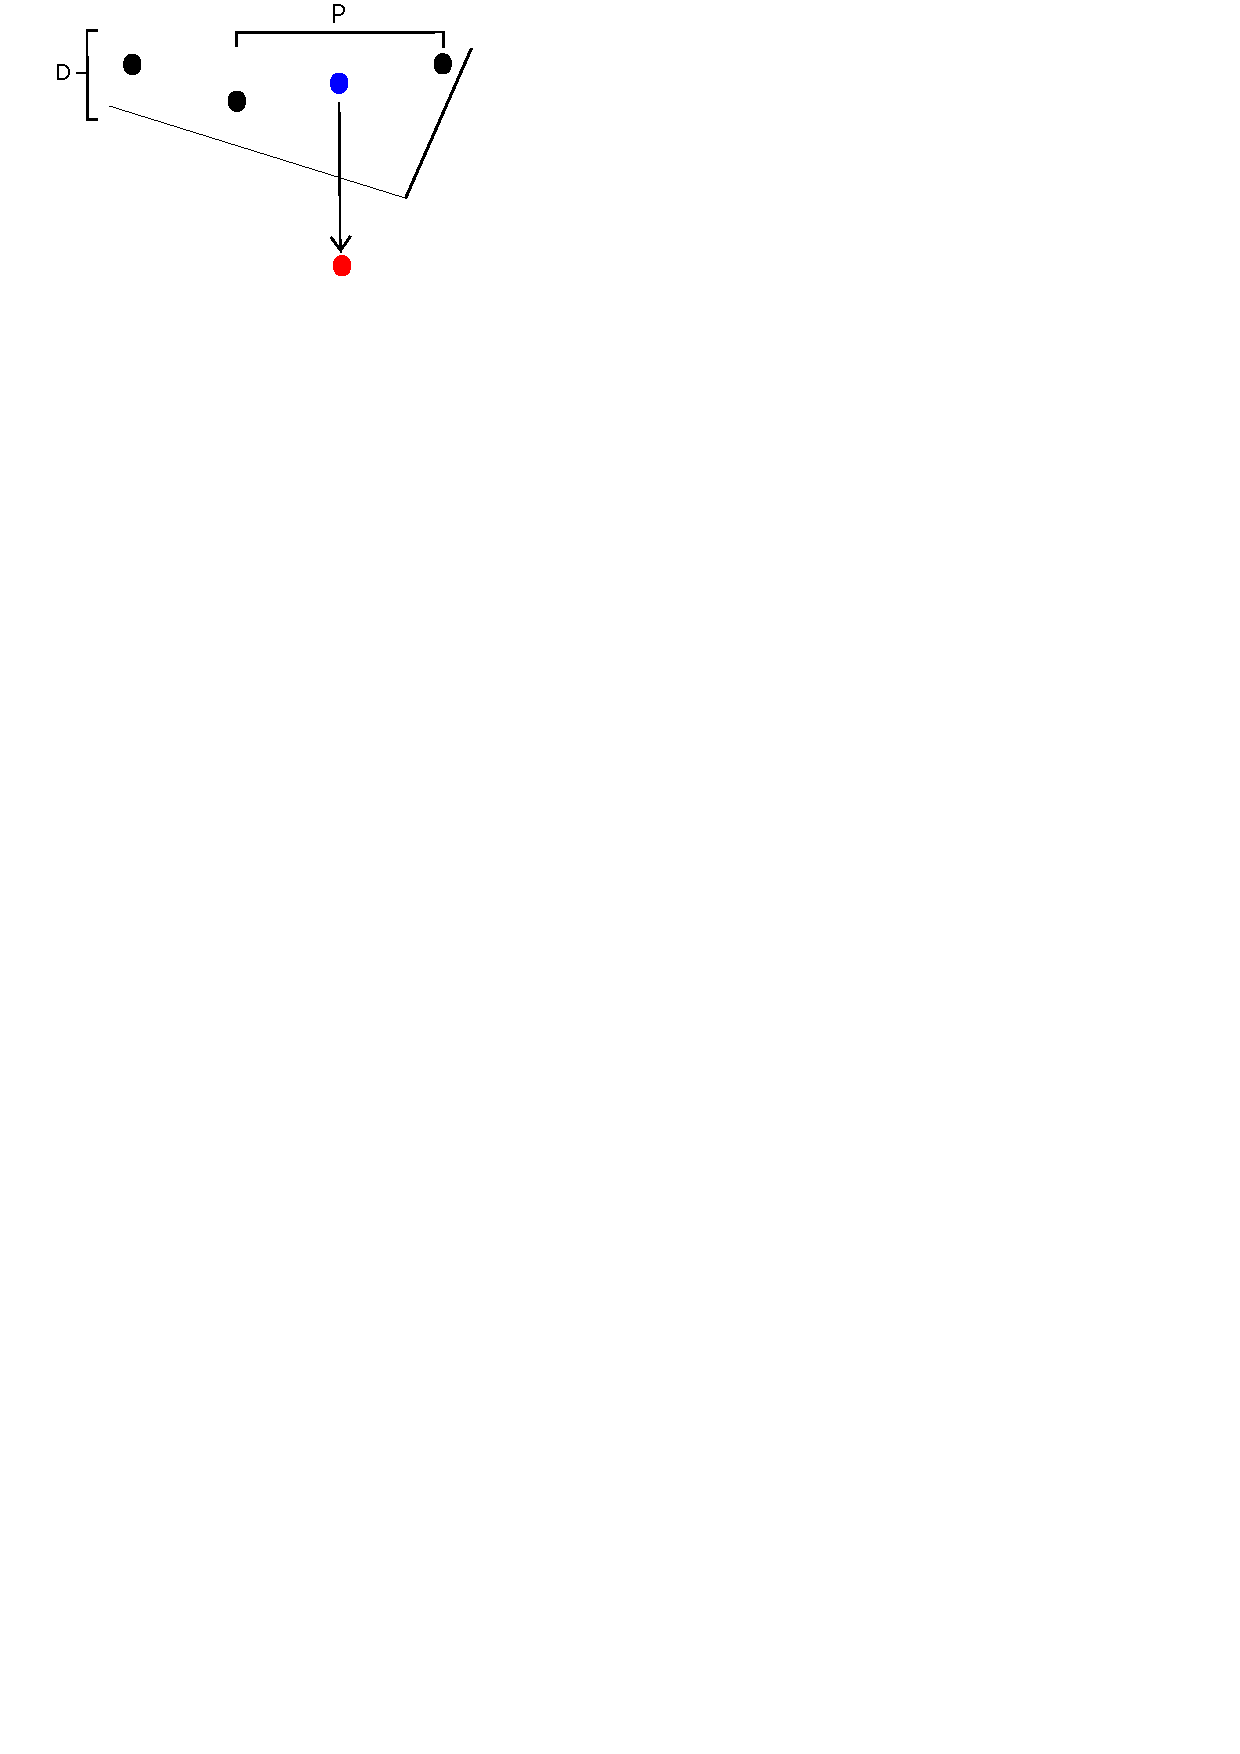
\includegraphics[trim={0 24cm 7cm 0}, clip, width=0.45\textwidth]{figures/artifs_theory2.pdf}\centering
	\caption{Another~illustration of an~artifact - the~black predictions are within the~maximum-error bound $D$, but the~blue one is not. The~blue prediction is shifted by $2D - 1$ to the~bottom, creating an~artifact.}
	\label{fig:artifs_theory}
\end{figure}

While the~prediction of the~order 2 filter is the~average of the~four neighboring values, the~prediction of the~order 4 filter tends to differ from the~neighboring values more, so this filter has the~tendency to produce more disturbing artifacts.

The~remaining pixels labeled $c$ are predicted from the~pixels $a\bullet$ and $b\bullet$ in $\ldot{i+1}$ by the~diagonally-oriented order 2 Neville interpolating filter (fig. \ref{fig:ccomp}). The~computation of residuals $\objnorm{E}{c}$ and $\objdot{E}{c}$ then follows according to the~target value $c_t$ from $\lnorm{i+1}$ and $c$ is assigned the~final value $c\bullet$ (eq. \ref{eq:b}).

\begin{figure}
	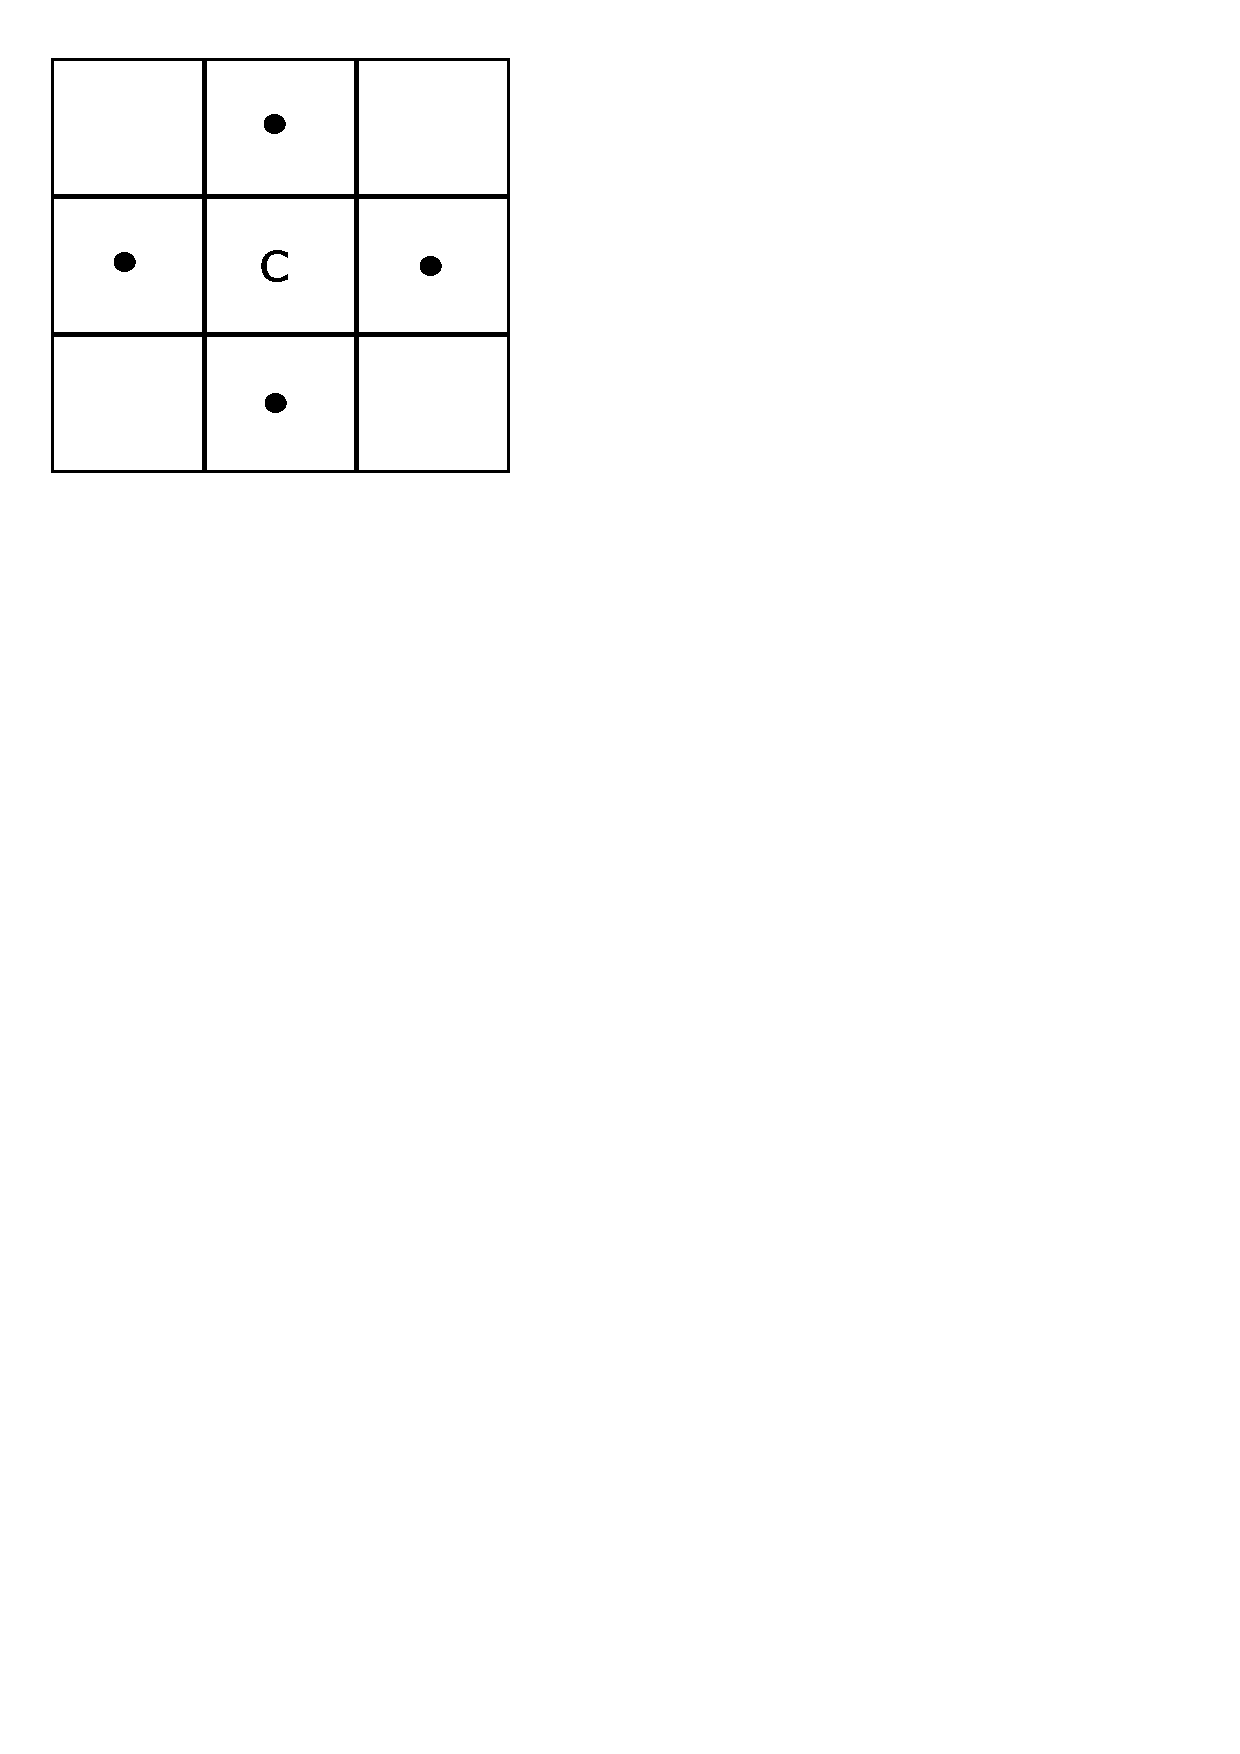
\includegraphics[trim={0 21cm 10cm 0}, clip, width=0.3\textwidth]{figures/ccomp.pdf}\centering
	\caption{The~prediction of $c$ - $\opnorm{P}{c}(\ldot{i+1})$ - is the~average of all the~pixels marked with a~dot - $\bullet$.}
	\label{fig:ccomp}
\end{figure}

$$\objnorm{E}{c} = c_t - \opnorm{P}{c}(\ldot{i+1})$$
$$\objdot{E}{c} = \opnorm{Q}{D}(\objnorm{E}{c})$$
\begin{equation}
\label{eq:c}
c\bullet = \opnorm{P}{c}(\ldot{i+1}) + \objdot{E}{c}
\end{equation}

The~cases when the~filter comes out of the~image are handled by a~specific mirror extension (fig. \ref{fig:cborders}). For the~same reasons as in the~prediction of $b$ pixels, the~order 2 filter is used for the~prediction of all $c$ pixels - both interior and exterior ones. Similarly, the~interpolation with such filter can be cached during diagonal traversal.

The~residuals $\objdot{E}{a}$, $\objdot{E}{b}$ and $\objdot{E}{c}$ are then encoded by an~entropy codec and stored. The~decompression is done in a~similar manner with the~only difference that the~residuals  are not computed anymore, but just decoded and read. So, we substitute every pixel from $\ldot{i}$ by four pixels in $\ldot{i+1}$, the~value of which is computed in three passes of prediction followed by adding the~read residual (the~last lines of eq. \ref{eq:a}, \ref{eq:b}, \ref{eq:c}).

\begin{figure}
	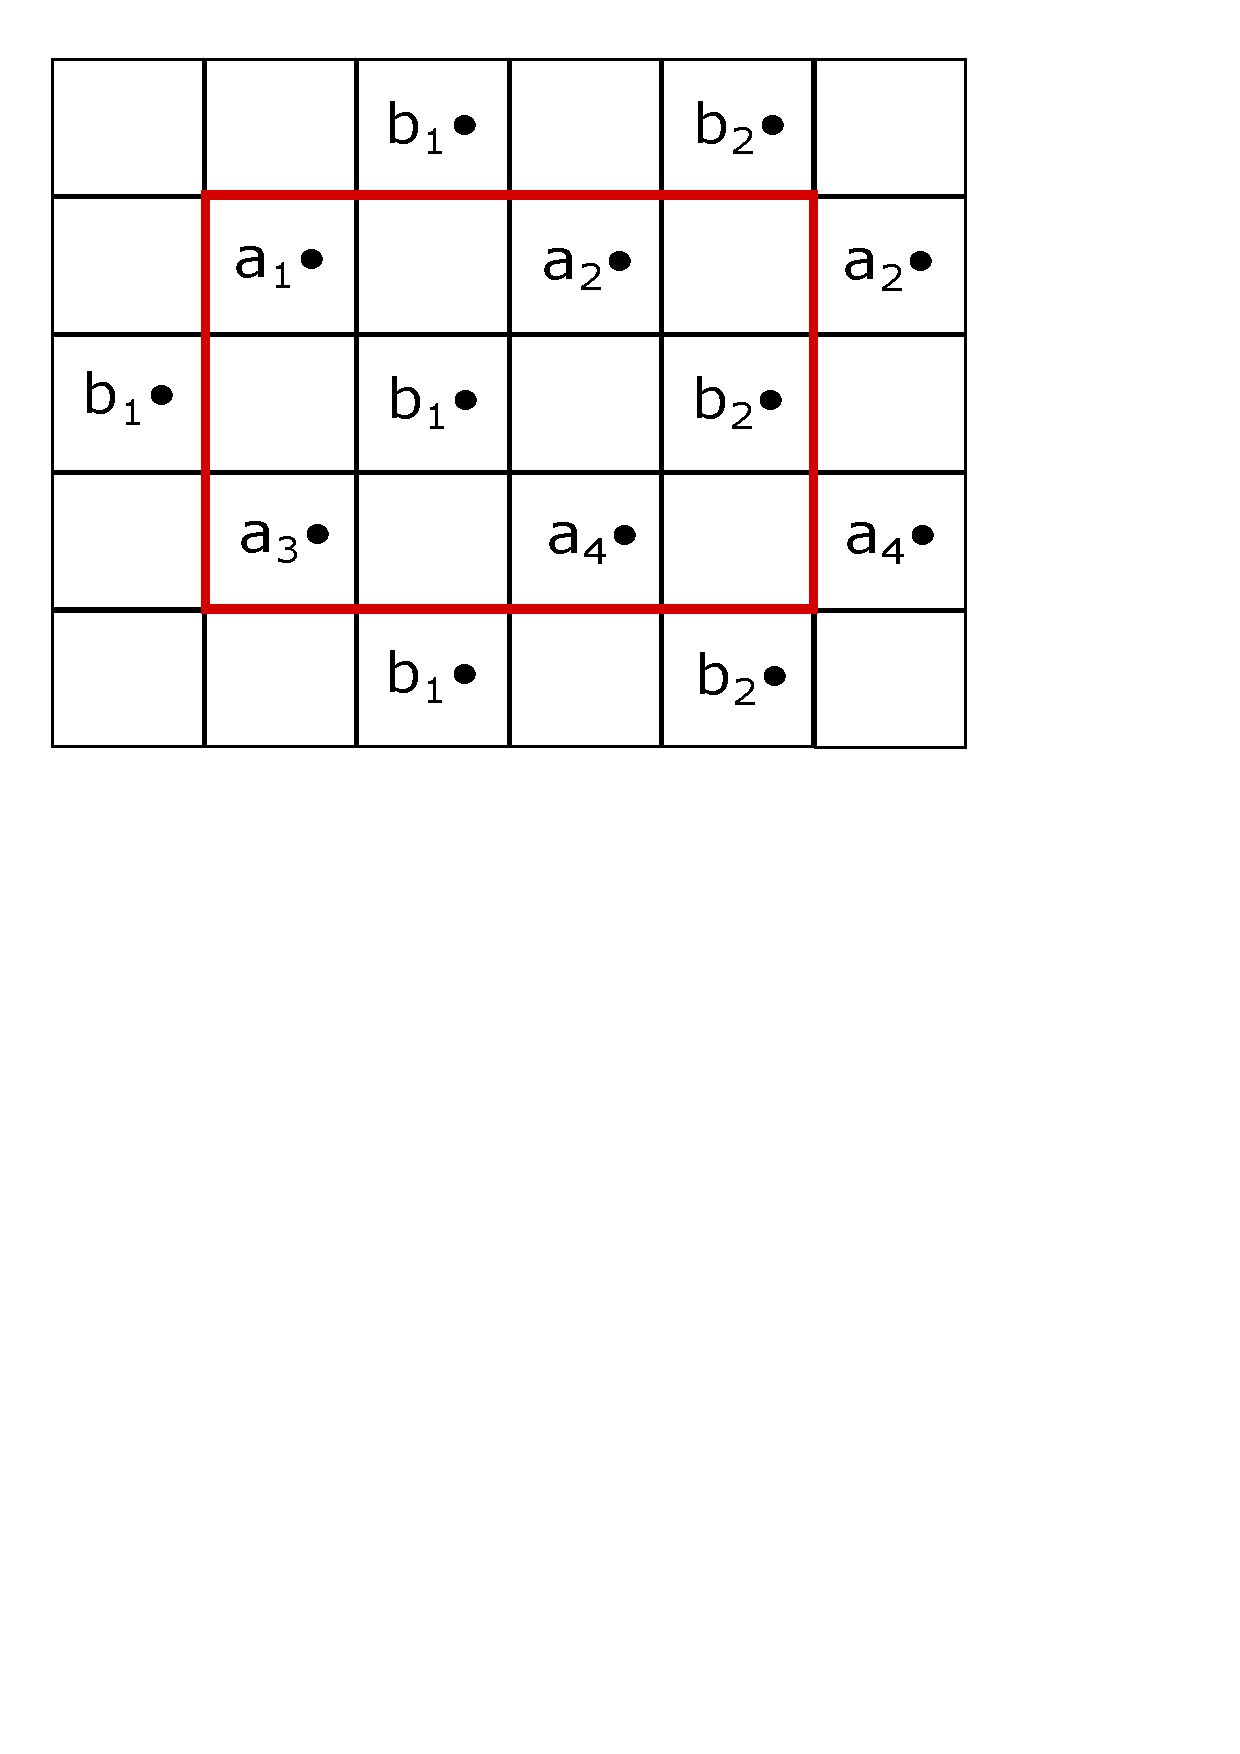
\includegraphics[trim={0 17cm 3cm 0}, clip, width=0.45\textwidth]{figures/extc.pdf}\centering
	\caption{Handling of border cases in the~computation of $\opnorm{P}{c}(\ldot{i+1})$ - the~red line represents the~border.}
	\label{fig:cborders}
\end{figure}